%
% Chapter 5
%
\chapter{Implementation}\label{chap:implementation}

The present chapter, will be developed and expanded upon in subsequent phases of the project, providing detailed insights into the implementation process and technical aspects of the solution.

\section{Mobile Application}\label{sec:mobile-application-implementation}

The mobile application layer, as previously mentioned at Section \ref*{sec:mobile-application}, is responsible for providing the user interface and interaction with the user. The application is developed using React Native\cite{ReactNativeBook} and Javascript\cite{Javascript} along with the Expo platform, which allows for the development of cross-platform applications, with a single codebase. The application is divided into several components, each responsible for a specific part of the application. The structure of the application is as follows:

\begin{itemize}
    \item \textbf{App} - Contains the main application files and folders such as authentication, navigation tabs, and initial screens.
    \item \textbf{Components} - Houses reusable UI components used throughout the application.
    \item \textbf{Assets} - Contains the images, icons, and colors used in the application.
    \item \textbf{Services} - Includes utility functions and services that handle tasks such as API calls and interaction with smart contracts.
\end{itemize}

\subsection{Application Structure and Design Philosophy}

The DiGo Certify mobile application is built on the principles of modularity, scalability, and maintainability. These principles guide the design and organization of the application, ensuring that each component is independent, reusable, and easy to maintain. The application leverages the Expo Router\cite{Expo-Router} for file-based routing, which provides a straightforward and efficient way to manage navigation within the app.

\subsubsection{File-Based Routing~\cite{Expo-Router-File-Based-Routing}}

File-based routing is a core feature of the Expo Router, allowing routes to be defined based on the file structure within the \texttt{app} directory. This approach simplifies the process of adding new routes and ensures a consistent and intuitive navigation structure. Each file or directory within the \texttt{app} directory represents a distinct route in the application.

For instance, the file \texttt{app/index.jsx} corresponds to the root route ("/"), and any additional files or nested directories create corresponding nested routes. This method provides a clear and organized way to manage the application's navigation, making it easy to understand and extend.

\begin{itemize}
    \item \textbf{Example:} Creating a new route is as simple as adding a new file. For example, adding a \texttt{details.jsx} file inside the \texttt{app} directory will create a new route accessible at "/details".
\end{itemize}

The \texttt{\_layout.jsx} file plays a crucial role in defining shared UI elements such as headers and footers that persist across different routes. This file acts as the root layout, ensuring a consistent look and feel throughout the application.

\subsubsection{Dynamic Routing}

Dynamic routing in Expo Router allows for more flexible navigation patterns by incorporating dynamic segments in the URL paths. This is particularly useful for routes that depend on parameters, such as user profiles or specific certificate details.

Dynamic segments are defined using square brackets in the file names. For example, a file named \texttt{[id].jsx} within a directory will match any URL segment, treating it as a variable. This allows the application to handle a wide range of dynamic routes efficiently.

\begin{itemize}
    \item \textbf{Example:} A route defined by \texttt{details/[id].jsx} can handle URLs like "/details/1" or "/details/2", where the segment after "/details/" is dynamic and can vary.
\end{itemize}

Expo Router's \texttt{Link} component is used to navigate between routes. It works similarly to the HTML \texttt{<a>} tag, using the \texttt{href} attribute to specify the target route. This component simplifies the process of linking different parts of the application, making the navigation seamless and intuitive.

\begin{itemize}
    \item \textbf{Example:} Using the \texttt{Link} component to navigate to a dynamic route can be done by passing the dynamic segment as a parameter: \texttt{<Link href="/details/1">View Details</Link>}.
\end{itemize}

\subsubsection{Advantages of File-Based and Dynamic Routing}

The combination of file-based and dynamic routing in Expo Router offers several advantages:

\begin{itemize}
    \item \textbf{Simplicity:} The file-based approach reduces the complexity of defining and managing routes, aligning with the project's philosophy of simplicity and maintainability.
    \item \textbf{Scalability:} As the application grows, new routes can be added easily by creating new files, making the application scalable without requiring significant changes to the existing structure.
    \item \textbf{Flexibility:} Dynamic routing allows for handling a wide range of navigation scenarios, providing the flexibility needed to support complex user interactions.
    \item \textbf{Consistency:} The use of layout files ensures that shared UI elements are consistently applied across different routes, providing a cohesive user experience.
\end{itemize}

In summary, the DiGo Certify application leverages the power of Expo Router's file-based and dynamic routing to create a robust, scalable, and maintainable navigation structure. This approach aligns with the overall design philosophy of the project, ensuring that the application is easy to extend, manage, and use.

\subsection{App Directory}

The \texttt{app} directory is the core of the application, containing the main screens and navigation setup. It is organized as follows:

\begin{itemize}
    \item \textbf{auth} - Manages the authentication flow.
    \item \textbf{tabs} - Handles the tab-based navigation within the application, such as Home, Profile, and Settings. This provides an intuitive way for users to navigate through different sections of the app.
    \item \textbf{initial-screen} - Contains the initial screen components displayed when the application is first launched. This includes splash screens and welcome messages that enhance the user onboarding experience.
    \item \textbf{\_layout.jsx} - Defines the layout structure of the application, including the header and footer components. This ensures a consistent look and feel across different screens.
    \item \textbf{emission.jsx} - Manages the certificate emission process, allowing administrators to issue new certificates. This is a critical component for the functionality of the DiGo Certify app.
    \item \textbf{index.jsx} - The entry point for the app directory, setting up the initial routing and navigation. This file integrates all the major components and initiates the application.
\end{itemize}

\subsection{Services Directory}

The services in the DiGo Certify frontend application play a crucial role in facilitating communication with the Ethereum blockchain and backend systems. Each blockchain interaction and backend microservice has a corresponding service in the frontend application, acting as a namespace that contains functions responsible for handling specific requests. These functions are asynchronous and return promises that resolve to the responses from these requests.

To interact with the Ethereum blockchain, the application utilizes the \texttt{ethers.js} library~\cite{ethers}, which provides a comprehensive set of tools for creating wallets, signing transactions, deploying smart contracts, and interacting with them. This library is chosen for its simplicity, robustness, and extensive documentation, making it ideal for handling blockchain operations within the application.

The \texttt{services} directory includes utility functions and services that handle tasks such as API calls, smart contract interactions, authentication processes, and secure storage. This directory is vital for maintaining clean and modular code, ensuring that the application's logic is well-organized and easily maintainable.

\subsubsection{Blockchain Services}

The \texttt{ethereum} directory within \texttt{services} handles interaction with the Ethereum blockchain, including smart contract calls. This service abstracts the complexity of blockchain interactions and provides simple methods for the application to use. Functions within this service manage tasks such as deploying contracts, invoking smart contract methods, and listening for events emitted by the contracts.

\subsubsection{Secure Storage}

Secure storage is a critical aspect of managing sensitive information within the application. The \texttt{storage.js} file within the \texttt{storage} directory leverages Expo's Secure Store~\cite{Expo-Secure-Store} to securely store sensitive data on the device. Expo Secure Store is a key-value storage system that encrypts data at rest, ensuring that sensitive information such as private keys and authentication tokens are stored securely.

\begin{itemize}
    \item \textbf{Expo Secure Store:} Provides a secure way to store sensitive key-value pairs on the device. It encrypts data at rest, making it a suitable choice for storing private keys and authentication tokens.
\end{itemize}

\subsubsection{WalletConnect Integration}

WalletConnect~\cite{Wallet-Connect} is integrated into the application to facilitate secure and user-friendly connections to Ethereum wallets. The \texttt{wallet-connect.js} file within the \texttt{web3} directory manages the WalletConnect integration. This service enables users to connect their Ethereum wallets to the DiGo Certify application, allowing for seamless interaction with the blockchain.

\begin{itemize}
    \item \textbf{WalletConnect:} A protocol that enables secure connections between the application and Ethereum wallets. It allows users to interact with the blockchain using their preferred wallet, enhancing the user experience and security.
\end{itemize}

\subsection{User Interface}

The user interface (UI) design of the DiGo Certify application focuses on simplicity, usability, and accessibility. The design principles are aimed at providing a seamless user experience that caters to the needs of all users, including students, alumni, and administrators.
The user journey diagram in Figure \ref{fig:user-journey} illustrates the key interactions and flows within the application, highlighting the various paths users can take to achieve their goals.

\begin{figure}[H]
    \centering
    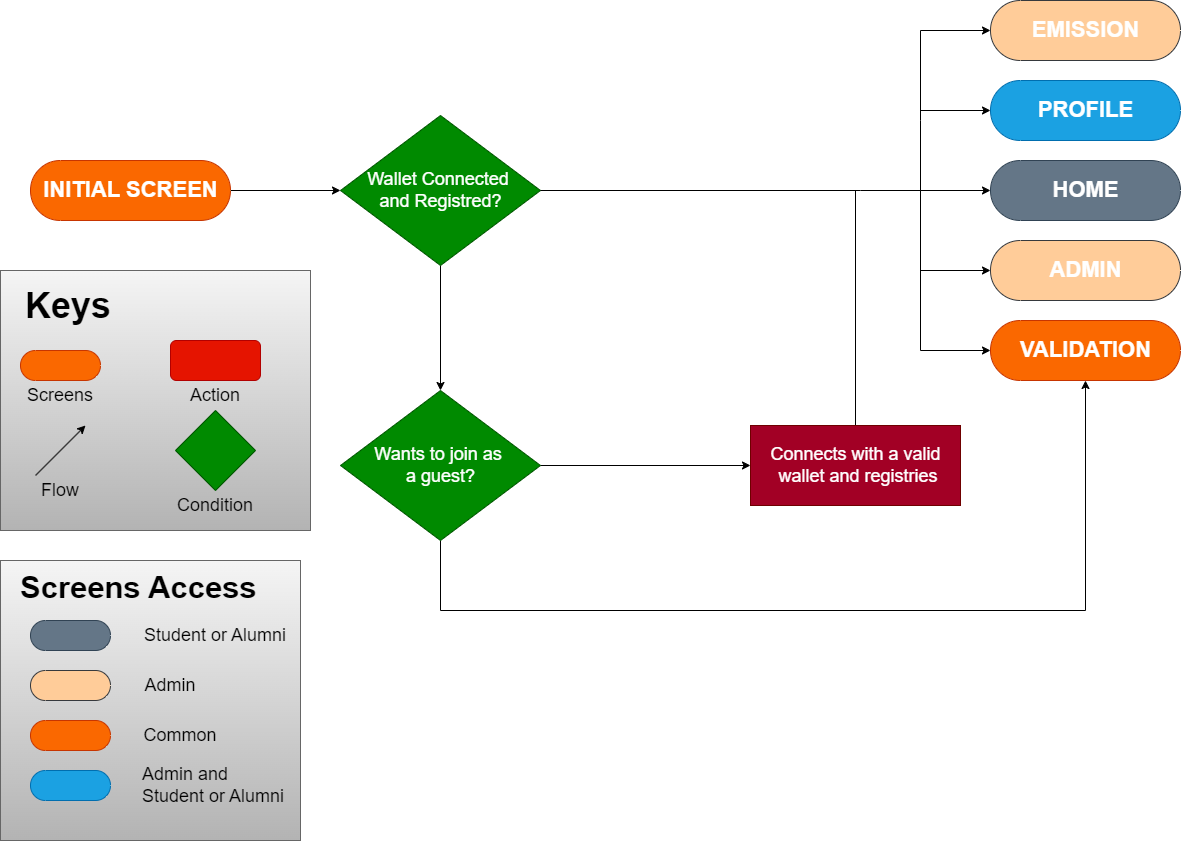
\includegraphics[width=0.7\textwidth]{./assets/app-flow.drawio.png}
    \caption{User Journey Diagram}
    \label{fig:user-journey}
\end{figure}

\section{Interaction with Smart Contracts}\label{sec:interaction-with-smart-contracts}
\paragraph{}

In this section we will briefly introduce the interaction between the DiGo Certify App and the Ethereum blockchain through smart contracts, outlining the importance of this interaction for the functionality of the application.

\subsection{Libraries and Tools for Blockhain Interaction}\label{subsec:utilizing-libraries-and-tools}
\paragraph{}

DiGo Certify App interacts with the smart contracts deployed on the Ethereum blockchain. The smart contracts are responsible for all the business logic of the application.
To make this interaction possible we used the \textit{ethers~\cite{ethers}} library which provides a set of tools to interact with the Ethereum blockchain, such as creating wallets, signing transactions, deploying smart contracts, and interacting with them~\cite{ethersDocs}.

The contracts that need to be present in the blockchain are deployed using \textit{Hardhat~\cite{hardhat}} that is a powerful Ethereum development environment that offers a comprehensive suite of tools for building, testing, and deploying smart contracts.
It provides an efficient and developer-friendly framework, streamlining the complex processes involved in Ethereum development. It offers a variety of features that are essential for modern blockchain development, such as
flexible plugin system~\cite{hardhatPlugins}, built-in tasks and scripts, hardhat network~\cite{hardhatNetwork}, smart contract debugging~\cite{hardhatDebug} and a good integration with the ethers library~\cite{hardhatWithEthers}.

\subsection{Managing Identities and Certificates}\label{subsec:managing-identities-and-certificates}
\paragraph{}

In our implementation, we leverage the \textbf{OnchainID~\cite{ONCHAINID}} and \textbf{Tokens for Regulated EXchanges~\cite{trexPurposeAndArchitecture}} contracts to manage identities, institutions, and certificates.
OnchainID is a blockchain-based identity system that identifies individuals and organisations, allowing them to enforce compliance and access digital assets~\cite{onchainidPruposalAndArchitecture}.
Their address is a unique identifier that can safely be used by a service provider to identify their owner and provide access to their services. Identities are smart contracts that support the ERC734: Key Manager~\cite{Vogelsteller_2017_key_manager} and ERC735: Key Holder~\cite{Vogelsteller_2017} standards, which define the structure of claims and keys, respectively.
The tools provided by OnchainID facilitate a secure, efficient, and scalable system for handling academic certificate emission onto the blockchain.
The OnchainID suite provides a comprehensive identity framework, ensuring that each participant in the ecosystem has a unique and verifiable identity
that can be used to issue, verify, and store academic credentials.
To simplify the deployment and management of identities, we use the \textit{IdentityFactory} contract from the OnchainID suite that follows the Factory pattern~\cite{harmes2008factory}, a design pattern recommended in the OnchainID documentation, which simplifies the creation and management of multiple instances of identities.
Every contract needed for the OnchainID is provided by a framework with the plugin \textbf{@onchain-id/identity-sdk} that was developed by the OnchainID team and provides easily import of the contracts.
On the other hand, T-REX does not provide a similar framework, so we had to import our own contracts to deploy the T-REX suite automated by the \textbf{deployTrexSuite} script.

The T-REX is a suite of blockchain-based solutions to issue and manage compliant security tokens on a distributed IT infrastructure. T-REX is Tokeny's implementation of the ERC3643 token standard used to manage institutions that issue certificates and the certificates themselves.
This suite provides a robust framework for handling the issuance and verification of academic credentials.
Similar to OnchainID, the T-REX suite utilizes the Factory pattern for creating and managing certificate-issuing contracts and also
use the Proxy pattern~\cite{harmes2008proxy} to create a proxy contract that acts as a gateway to the certificate-issuing contracts, allowing for upgrades to the certificate management logic without disrupting existing data.
This ensures that the system remains adaptable to future changes and improvements.
The T-REX suite includes registries for trusted issuers that work similarly as a Whitelist, allowing that only verified institutions that are present in the registry can issue certificates. This registry is crucial for maintaining the system's integrity, as it prevents unauthorized entities from issuing fraudulent certificates.

\subsection{Contract Interaction Setup}\label{subsec:interacting-with-the-contracts}
\paragraph{}

To be able to interact with the contracts, hardhat compile and stores the contract's ABI (Application Binary Interface) and the contract's address in a JSON file that is generated before launching the application by the auxiliary script \textbf{install.sh}.
The ABI is a JSON representation of the contract's interface, which includes the functions, events, and variables of the contract. The address is the location of the contract on the blockchain.

After the contracts are deployed, the application interact with them using the \textit{ethers.js} library and a set of helper functions that were created to facilitate the interaction with the contracts (e.g \textbf{getContractAt}, \textbf{getWallet}\dots).
These functions are located in the \textit{utils} folder of the ethereum services and are imported in the necessary components.

\section{Smart Contracts}\label{sec:smart-contracts-implementation}
\paragraph{}

In this section we offer a thorough description of the implementation of the most important smart contracts used in the system. For more detailed information about the app architecture, consult Section~\ref{sec:fully-distributed-environment}.
The core of the services provided by the DiGo Certify App is the management of digital identities and certificates on the blockchain and they are implemented in the \textbf{ethereum} folder of the project with the following structure:

\begin{itemize}
    \item \textbf{contracts}: Contains the smart contracts deployed on the blockchain.
    \item \textbf{scripts}: Houses functions responsible for automating blockchain operations, such as contract deployment and interaction.
          \subitem\textbf{identities}: Functions related to the management of digital identities.
          \subitem\textbf{claimIssuer}: Functions pertaining to institutions that issue certificates.
          \subitem\textbf{claims}: Functions associated with the issuance of certificates.
          \subitem\textbf{suites}: Functions for deploying the OnchainID and T-REX suites.
          \subitem\textbf{utils}: Helper functions utilized throughout the application.
    \item \textbf{test}: Includes test scripts and cases validating the functionality of contracts and scripts.
\end{itemize}

\subsection{Institution Creation}\label{subsec:creating-institutions}
\paragraph{}

In this section, we discuss the process of creating institutions, known within the DiGo Certify App as Claim Issuers, on the Ethereum blockchain.
Claim Issuers are entities that have the authority to issue certificates to students and alumni. The creation of Claim Issuers is a crucial step in the certification validation process, as it ensures that only verified institutions can issue certificates.
The Claim Issuer creation process is automated through the use of the \textbf{deployClaimIssuer} function, which is responsible for deploying a new Claim Issuer contract associated with a specified wallet address.

The function begins by deploying into the blockchain a new Claim Issuer contract for the specified address and waits until the block is mined in order to retrieve the deployed contract instance.
After the Claim Issuer contract deployment, we access the \textbf{TrustedIssuerRegistry} contract, which is the Whitelist of trusted issuers, and add the new Claim Issuer to the registry making the new
Claim Issuer a trusted entity that can issue certificates. This is done by calling the \textbf{addTrustedIssuer} function of the TrustedIssuerRegistry contract, which requires the Claim Issuer address and a predefined list of permitted claim topics. See with more detail in Section~\ref{subsubsec:understanding-claims-and-certificates}.
After being in the whitelist, the institution self assign his institution code for future identification and reference within the application.
In the end the claim issuer contract address, abi, institution code and both public and private keys are stored in the configuration file.

This entire process is managed through a shell script, accessible exclusively to the owner of the DiGo Certify App. This measure ensures that only authorized personnel can initiate and oversee the creation of new Claim Issuers, maintaining the integrity and security of the certification issuance framework.

\subsection{Identity Creation}\label{subsec:creating-identities}
\paragraph{}

The first step in the process of the certification validation process is the creation of a student identity. After the registration process at the beginning of the app, the student's identity is created on the blockchain.
This is done by calling the \textbf{deployIdentity} function that contains all the necessary logic to create a new identity. The primary objective of this function is to automate the process of deploying a new identity contract associated with a specified wallet address.
It begins by validating inputs such as the wallet address and a unique cryptographic salt used for identity creation, ensuring that the identity is unique. This is a read-write operation
that requires to be signed by the owner private key. Upon successful deployment the function monitors the blockchain for relevant events, such as \textbf{WalletLinked} to confirm the identity creation.

Once created the function retrieves the deployed identity contract instance that allows subsequent interactions and operations with the newly created identity contract.

\subsection{Asking for a Certificate}\label{subsec:asking-for-a-certificate}
\paragraph{}

After having a digital identity created on the blockchain it's possible to ask for a certificate. Before the procedure of asking a certificate, it is necessary to have knowledge how a request for a certificate translates into the blockchain operations.

\subsubsection*{Understanding Claims and Certificates}\label{subsubsec:understanding-claims-and-certificates}
\paragraph{}

In the DiGo Certify App, certificates are represented as claims how was introduced in Section~\ref{subsec:managing-identities-and-certificates}.
A claim is a statement or assertion made by a Claim Issuer about an identity, such as a student name, date of birth, etc.
In the context of our application, a claim is used not only to represent a statement about the identity but also to represent a unique digital asset~\cite{enwiki:1234201704} that can be issued and verified on the blockchain.
Claims can be obtained by several sources, such as the \textit{Identity Owner}, known as \textbf{´self attested'} claims or anyone that the identity owner allowed to issue claims on his behalf, known as ´delegated' claims. This
identity allowed to issue claims is typically an institution that has been added to the TrustedIssuerRegistry. The function \textbf{addKeyToIdentity} is used to manage the keys that are allowed to issue claims on behalf of the identity owner. This function is called by the identity owner and requires the key of the institution that is allowed to issue claims.

Claims may be related to sensitive data. Despite what legislation says about data privacy, in our solution we are storing the public data directly on the blockchain for easily access from both parts, the identity owner and the claim issuer.
However the data that need to be kept private is hashed before being stored, using the SHA-256 algorithm and a symmetric key that is only known by the identity owner and the claim issuer. This way, the data is kept private and only the parts that need to be public are stored in plain text.
A claim has the following structure:
\begin{itemize}
    \item \textbf{data}: The data of the claim, such as the student name, student number, course code;
    \item \textbf{topic}: The topic of the claim. [INSTITUTION, STUDENT, CERTIFICATE];
    \item \textbf{issuer}: The address of the claim issuer;
    \item \textbf{signature}: The signature of the claim issuer (function \textbf{signMessage} is used to sign the claim on behalf of the claim issuer wallet);
    \item \textbf{shceme}: The scheme of the claim, such as ECDSA, RSA, etc;
    \item \textbf{claimId}: The unique identifier of the claim that is generated by the claim issuer;
    \item \textbf{uri}: Where the claim is stored or the hash of the claims
\end{itemize}

\paragraph{}

The process of asking for a certificate is done after the user has inserted all the necessary information in the app, such as the institution code, name and student number.
Then the function \textbf{getTrustedIssuersForClaimTopic} is called to get the list of trusted issuers that are allowed to issue claims for the specified topic.
After the correct claim issuer is found, the function \textbf{addClaim} is called after the key of the institution is added to student's identity. This function is called two times
and creates two self-attested claims, one for the student name and other for the student number.

\subsection{Certificate Issuance}\label{subsec:certificate-issuance}
\paragraph{}

The issuance of certificates by a trusted institution is very similar to the process of asking for the certificate described in the Section~\ref{subsec:asking-for-a-certificate}.
The main difference is that the claim issuer sends some other claims to the student's identity, such as the course code, the course conclusion date, the course code, the certificate registration number and the certificate.
As we described in Section~\ref{subsubsec:understanding-claims-and-certificates}, the certificate is stored privately in the blockchain in two ways. The first is the hash of the certificate that is stored in the blockchain and the second is the hash of certificate is stored.
The certificate can be accessed by the student using the key that the he sent to the claim issuer when asking for the certificate.

If there is a need to change the certificate, the institution can send a new certificate to student's identity and the claims will be updated.

\subsection{Certificate Validation}\label{subsec:certificate-verification}
\paragraph{}

The validation of certificates is the main feature of the DiGo Certify App and at the same time the most easy to implement. To make this, there's no need to have an identity created on the blockchain, only the certificate hash and the student address are needed.
The function \textbf{makeValidation} is called with the certificate hash and the student address and the function returns if the hash of the certificate is the same as the hash stored in the claims of the student's identity.
